\documentclass[12pt,a4paper]{article}

% =========================================================
%  CSE 3205 Assignment (Single-file LaTeX)
%  Color Design + Graph + GitHub link
% =========================================================

\usepackage[a4paper,margin=1in]{geometry}
\usepackage[T1]{fontenc}
\usepackage{lmodern}
\usepackage{microtype}

\usepackage{graphicx}
\usepackage{float}
\usepackage{amsmath}
\usepackage{enumitem}
\usepackage{booktabs}
\usepackage{array}
\usepackage{colortbl}

% ---------- Colors & Design ----------
\usepackage{xcolor}
\usepackage{titlesec}
\usepackage{fancyhdr}
\usepackage{tcolorbox}

% ---------- Links ----------
\usepackage[hidelinks]{hyperref}
\hypersetup{
  colorlinks=true,
  linkcolor=blue,
  urlcolor=blue,
  citecolor=blue
}

% ---------- Graphs ----------
\usepackage{tikz}
\usepackage{pgfplots}
\pgfplotsset{compat=1.18}

% ---------- Optional QR (uncomment if you want QR code) ----------
% \usepackage{qrcode}

% ---------- Lists ----------
\setlist[itemize]{noitemsep, topsep=3pt}
\setlist[enumerate]{noitemsep, topsep=3pt}

% ---------- Theme Colors ----------
\definecolor{Primary}{HTML}{1F4E79}   % deep blue
\definecolor{Accent}{HTML}{2E7D32}    % green
\definecolor{Soft}{HTML}{F3F6FA}      % light gray-blue
\definecolor{TableHead}{HTML}{D9E2EF} % table header

% ---------- Section styling ----------
\titleformat{\section}
  {\Large\bfseries\color{Primary}}{\thesection}{0.8em}{}
\titleformat{\subsection}
  {\large\bfseries\color{Accent}}{\thesubsection}{0.8em}{}
\titleformat{\subsubsection}
  {\normalsize\bfseries\color{Primary}}{\thesubsubsection}{0.8em}{}

% ---------- Header/Footer ----------
\pagestyle{fancy}
\fancyhf{}
\lhead{\color{Primary}\textbf{CSE 3205: Software Engineering}}
\rhead{\color{Primary}\textbf{Assignment}}
\cfoot{\color{Primary}\thepage}
\renewcommand{\headrulewidth}{0.6pt}
\renewcommand{\headrule}{\hbox to\headwidth{\color{Primary}\leaders\hrule height \headrulewidth\hfill}}

% ---------- Boxes ----------
\newtcolorbox{infobox}[1]{
  colback=Soft,
  colframe=Primary,
  title=\textbf{#1},
  fonttitle=\color{Primary},
  arc=3mm,
  boxrule=0.8pt
}
\newtcolorbox{keypoint}{
  colback=white,
  colframe=Accent,
  arc=2mm,
  boxrule=0.7pt
}

% ---------- Table row colors ----------
\rowcolors{2}{Soft}{white}

% =========================================================
%  STUDENT INFORMATION (FILLED)
% =========================================================
\newcommand{\StudentName}{Arif Foysal Bin Haider}
\newcommand{\StudentRoll}{2103119}
\newcommand{\StudentSection}{B}
\newcommand{\StudentSeries}{21}
\newcommand{\TeacherName}{Md.\ Sozib Hossain}
\newcommand{\SubmissionDate}{12 February 2026}

% Put your GitHub repository link here:
\newcommand{\GitHubLink}{https://github.com/your-username/your-repo} % <-- EDIT THIS

\begin{document}

% =========================================================
%  COVER PAGE
% =========================================================
\begin{titlepage}
\centering
\vspace*{0.4cm}

{\Large \textbf{Heaven's Light is Our Guide}\par}
\vspace{0.2cm}
{\Large \textbf{Rajshahi University of Engineering \& Technology (RUET)}\par}
\vspace{0.2cm}
{\large Department of Computer Science \& Engineering\par}

\vspace{1.0cm}
{\LARGE \textbf{Assignment}\par}
\vspace{0.7cm}

{\large \textbf{``Software Process Models, Software Testing \& Quality Assurance, and Design Patterns \& Modern Software Tools''}\par}

\vspace{0.9cm}

\begin{tabular}{>{\bfseries}l l}
Course Code & : CSE 3205\\
Course Title & : Software Engineering\\
Date of Submission & : \SubmissionDate\\
\end{tabular}

\vspace{1.0cm}

\begin{infobox}{GitHub Repository (Code Reference)}
\textbf{Link:} \href{\GitHubLink}{\url{\GitHubLink}}\\
(Teacher can review implementation, diagrams source, tests, and version history.)
\end{infobox}

% Optional QR code:
% \vspace{0.4cm}
% \qrcode[height=2.8cm]{\GitHubLink}

\vfill

\begin{minipage}{0.45\textwidth}
\textbf{Submitted by}\\[6pt]
Name : \StudentName\\
Roll : \StudentRoll\\
Section : \StudentSection\\
Series : \StudentSeries\\
\end{minipage}
\hfill
\begin{minipage}{0.45\textwidth}
\textbf{Submitted to}\\[6pt]
\TeacherName\\
Lecturer\\
Department of CSE, RUET\\
\end{minipage}

\vspace{0.8cm}
\end{titlepage}

\tableofcontents
\newpage

% =========================================================
%  ASSIGNMENT 1
% =========================================================
\section{Assignment 1: Software Process Models Analysis}

\subsection{Scenario Overview}
A mid-sized software company plans to build an Online Course Management System (OCMS) that will
continuously evolve with frequent requirement changes. Since the platform must remain market-relevant,
it requires continuous user feedback (from students, instructors, and administrators). Therefore, the chosen
process model should emphasize iterative delivery, controlled change handling, and stakeholder collaboration.

\subsection{1. Process Model Identification \& Analysis}

\subsubsection{Model 1: Agile (Scrum)}
\textbf{Core characteristics}
\begin{itemize}
  \item \textbf{Iterative \& incremental}: Work is delivered in short sprints (typically 1--4 weeks).
  \item \textbf{Feedback loops}: Sprint review and sprint retrospective happen in every sprint.
  \item \textbf{Change management}: Product Backlog is reprioritized between sprints to accommodate change.
\end{itemize}

\textbf{How it fits OCMS}
\begin{itemize}
  \item Early sprints can deliver basic modules (login, course listing) while later sprints add enrollment,
        grading, analytics, etc.
  \item Stakeholders can test working software frequently and suggest improvements immediately.
\end{itemize}

\subsubsection{Model 2: Spiral Model}
\textbf{Core characteristics}
\begin{itemize}
  \item \textbf{Risk-driven iteration}: Each cycle includes planning, risk analysis, development, and evaluation.
  \item \textbf{Prototyping}: Reduces uncertainty when requirements are unclear or changing.
  \item \textbf{Formal control}: Better documentation and explicit risk mitigation compared to Agile.
\end{itemize}

\textbf{How it fits OCMS}
\begin{itemize}
  \item Strong when the project has significant risks (complex integrations, security, scaling).
  \item Changes are incorporated through re-planning at the beginning of each spiral.
\end{itemize}

\subsection{2. Comparative Engineering Analysis}

\begin{table}[H]
\centering
\caption{Agile (Scrum) vs Spiral Model for OCMS (engineering comparison)}
\begin{tabular}{p{3.4cm} p{5.8cm} p{5.8cm}}
\toprule
\rowcolor{TableHead}
\textbf{Metric} & \textbf{Agile (Scrum)} & \textbf{Spiral Model}\\
\midrule
Requirement Flexibility &
Very high: backlog reprioritization each sprint supports frequent changes with minimal disruption. &
High but slower: changes absorbed per spiral; longer cycles can delay updates.\\
\addlinespace
Risk Management &
Moderate: risks handled through continuous integration/testing and early validation (implicit). &
Very strong: explicit risk identification and mitigation in every spiral iteration.\\
\addlinespace
Customer Involvement &
High and frequent: sprint reviews enable continuous feedback on working software. &
High but milestone-based: evaluation at spiral end; typically less frequent.\\
\addlinespace
Development Cost &
Lower overhead; rework cost reduced by short cycles and early feedback. &
Higher overhead due to risk analysis and documentation; cost-effective mainly for high-risk projects.\\
\addlinespace
Predictability &
Flexible; progress tracked empirically using sprint velocity and burn-down. &
More milestone predictability due to structured planning per spiral.\\
\bottomrule
\end{tabular}
\end{table}

\subsection*{Visual Comparison (Graph)}
\begin{figure}[H]
\centering
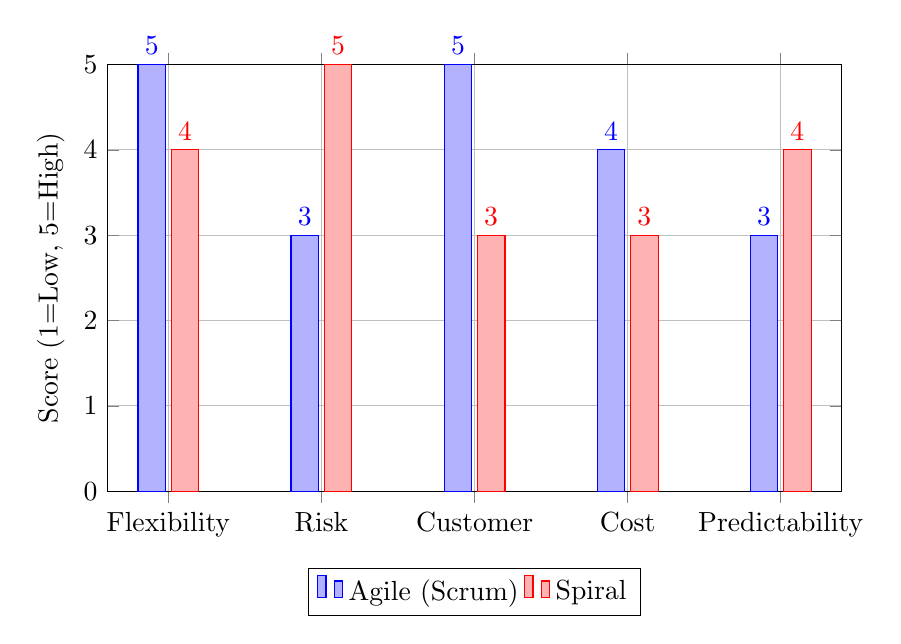
\begin{tikzpicture}
\begin{axis}[
    ybar,
    bar width=10pt,
    width=0.9\textwidth,
    height=7cm,
    ymin=0, ymax=5,
    ylabel={Score (1=Low, 5=High)},
    symbolic x coords={Flexibility,Risk,Customer,Cost,Predictability},
    xtick=data,
    legend style={at={(0.5,-0.18)},anchor=north,legend columns=2},
    nodes near coords,
    nodes near coords align={vertical},
    grid=both
]
\addplot coordinates {(Flexibility,5) (Risk,3) (Customer,5) (Cost,4) (Predictability,3)};
\addplot coordinates {(Flexibility,4) (Risk,5) (Customer,3) (Cost,3) (Predictability,4)};
\legend{Agile (Scrum),Spiral}
\end{axis}
\end{tikzpicture}
\caption{Agile vs Spiral (relative scoring for this scenario)}
\end{figure}

\subsection{3. Justification \& Recommendation}

\begin{infobox}{Recommendation}
\textbf{Selected Model: Agile (Scrum)}\\
Agile is recommended because it best supports frequent requirement changes, continuous feedback, and
fast incremental delivery---which is ideal for a mid-sized company building an evolving OCMS.
\end{infobox}

\textbf{Justification}
\begin{itemize}
  \item \textbf{Frequent requirement changes:} sprint-based planning absorbs changes every few weeks.
  \item \textbf{Continuous user feedback:} sprint reviews ensure the product remains aligned with market needs.
  \item \textbf{Mid-sized company fit:} avoids the heavy risk-documentation overhead that Spiral often requires.
  \item \textbf{Early MVP:} enables early release and improvement based on real usage data.
\end{itemize}

\newpage

% =========================================================
%  ASSIGNMENT 2
% =========================================================
\section{Assignment 2: Software Testing \& Quality Assurance Plan}

\subsection{Scenario Overview}
A Library Management System (LMS) supports searching books, borrowing/returning items, and managing
user accounts. Reliability and data accuracy are critical because incorrect inventory status, wrong fines,
or broken transactions can disrupt library operation.

\subsection{1. Test Strategy Design (Four Testing Types)}

\begin{table}[H]
\centering
\caption{Testing types and purpose statements}
\begin{tabular}{p{3.2cm} p{12.0cm}}
\toprule
\rowcolor{TableHead}
\textbf{Testing Type} & \textbf{Purpose}\\
\midrule
Unit Testing & Validates individual functions/methods (fine calculation, ISBN validation) in isolation.\\
Integration Testing & Validates interactions between modules (borrow service $\leftrightarrow$ DB update $\leftrightarrow$ user record).\\
System Testing & Validates the complete integrated system end-to-end under realistic conditions.\\
Acceptance Testing (UAT) & Confirms real users (librarian/patron/admin) can complete workflows and the system meets business rules.\\
\bottomrule
\end{tabular}
\end{table}

\subsection{2. Example Test Scenarios}

\subsubsection{Unit Test Scenario}
\textbf{Function:} \texttt{CalculateOverdueFine(borrowDate, returnDate, periodDays)} (period=14 days, rate=\$0.50/day)
\begin{itemize}
  \item borrow=Jan 1, return=Jan 21 $\Rightarrow$ overdue=6 days $\Rightarrow$ fine=\$3.00
  \item borrow=Jan 1, return=Jan 10 $\Rightarrow$ fine=\$0.00
  \item returnDate = null $\Rightarrow$ throws InvalidDateException
\end{itemize}

\subsubsection{Integration Test Scenario}
\textbf{Modules:} Borrowing $\leftrightarrow$ Inventory DB $\leftrightarrow$ User Account
\begin{itemize}
  \item Borrow available book $\Rightarrow$ create borrow record + decrement copies by 1
  \item If copies=0 $\Rightarrow$ borrowing is blocked
  \item If DB fails $\Rightarrow$ no partial update persists (transaction rollback)
\end{itemize}

\subsubsection{System Test Scenario}
\textbf{Workflow:} Login $\rightarrow$ Search $\rightarrow$ Borrow $\rightarrow$ Return
\begin{itemize}
  \item State updates are correct (availability, borrow history, due date)
  \item Each operation responds in $<2$ seconds under normal load
  \item Concurrent borrow of last copy: only one succeeds; others receive ``Unavailable''
\end{itemize}

\subsubsection{Acceptance Test (UAT) Scenario}
\textbf{User:} Librarian
\begin{itemize}
  \item Scan barcode $\rightarrow$ system finds borrower $\rightarrow$ calculates fine $\rightarrow$ marks Available
  \item Fine matches manual calculation (if overdue), and book becomes searchable immediately
\end{itemize}

\subsection{3. Software Quality Assurance (SQA) Plan}

\subsubsection{Quality Goals (Measurable Metrics)}
\begin{table}[H]
\centering
\caption{SQA measurable targets}
\begin{tabular}{p{4.0cm} p{6.3cm} p{4.8cm}}
\toprule
\rowcolor{TableHead}
\textbf{Quality Attribute} & \textbf{Metric} & \textbf{Target}\\
\midrule
Reliability & System uptime & 99.9\% uptime\\
Critical Defects & Severity-1 defects in production & 0\\
Data Accuracy & Inventory/account mismatch rate & 0 critical mismatches; accuracy $\geq$ 99.99\%\\
Performance & Search response time & $<2$ seconds for 95\% of queries\\
Defect Leakage & Critical bugs found after release & 0\\
Test Coverage & Automated line coverage & $\geq$ 85\% (100\% for critical modules)\\
\bottomrule
\end{tabular}
\end{table}

\subsubsection{Review \& Testing Activities}
\begin{table}[H]
\centering
\caption{When reviews and testing occur}
\begin{tabular}{p{3.5cm} p{10.8cm}}
\toprule
\rowcolor{TableHead}
\textbf{Phase} & \textbf{Activities}\\
\midrule
Requirements & Review for completeness, consistency, and testability.\\
Design & Review DB schema, API contracts, UI flows before implementation.\\
Implementation & Code review for every pull request; static analysis on commits.\\
Testing & Unit $\rightarrow$ Integration $\rightarrow$ System tests; regression suite runs regularly.\\
Pre-release & UAT in staging with representative librarian/patron scenarios.\\
Post-release & Monitoring: error rates, logs, performance dashboards, health checks.\\
\bottomrule
\end{tabular}
\end{table}

\subsubsection{Defect Tracking Approach}
\begin{infobox}{Defect Lifecycle (with triage)}
New $\rightarrow$ Triaged $\rightarrow$ Assigned $\rightarrow$ In Progress $\rightarrow$ Fixed $\rightarrow$ Retest $\rightarrow$ Verified $\rightarrow$ Closed
\end{infobox}

\textbf{Severity levels:}
\begin{itemize}
  \item \textbf{Critical:} crash/data loss/security breach (fix within 24 hours)
  \item \textbf{High:} major function broken (fix within sprint)
  \item \textbf{Medium/Low:} minor functional/usability/cosmetic (schedule)
\end{itemize}

\subsection{4. Impact Evaluation}
This strategy improves reliability and user satisfaction by catching defects early (unit testing),
preventing interface/transaction failures (integration testing), validating end-to-end workflows (system testing),
and ensuring business-rule compliance through real user checks (UAT). Measurable SQA targets and a structured
defect lifecycle reduce downtime, improve data correctness, and increase trust.

\newpage

% =========================================================
%  ASSIGNMENT 3
% =========================================================
\section{Assignment 3: Design Patterns \& Modern Software Tools}

\subsection{Scenario Overview}
A Smart Home Automation System manages dynamically created devices (lights, fans, sensors) and controls them
centrally. The design must remain scalable and flexible as device types and vendors expand over time.

\subsection{1. Architectural Pattern Selection}
\textbf{Selected Pattern: Abstract Factory Pattern.}

\begin{infobox}{Why Abstract Factory?}
It supports dynamic creation of \textbf{families of related device objects} (e.g., vendor/protocol-based)
without specifying concrete classes in the controller, enabling centralized management with loose coupling.
\end{infobox}

\subsection*{Diagram (Insert your Draw.io image)}
Export a class diagram from Draw.io (PNG) and insert it here using \texttt{\textbackslash includegraphics}.
\begin{figure}[H]
\centering
\fbox{\parbox{0.9\textwidth}{
\textbf{Diagram Guide (Abstract Factory):}\\
SmartDeviceFactory interface: createLight(), createFan(), createSensor()\\
Concrete factories: PhilipsFactory, XiaomiFactory, etc.\\
Product interfaces: Light, Fan, Sensor\\
Concrete products per family: PhilipsLight, XiaomiLight, etc.\\
SmartHomeController uses only interfaces and keeps a device list for central control.
}}
\caption{Abstract Factory applied to Smart Home Automation (insert diagram)}
\end{figure}

\subsection{2. Engineering Justification}
\begin{itemize}
  \item \textbf{Scalability:} add new device types/families by extending factories and product classes; controller unchanged.
  \item \textbf{Maintainability:} creation/initialization logic stays in factory classes, isolating vendor changes.
  \item \textbf{Flexibility:} runtime factory selection allows different vendors/configurations without rewriting core logic.
\end{itemize}

\subsection{3. Comparative Analysis}
\textbf{Alternative: Simple Factory / Direct Instantiation.} Direct creation (e.g., \texttt{new Light()})
couples controller to concrete classes, making expansion harder and increasing modification risk.

\begin{table}[H]
\centering
\caption{Abstract Factory vs Simple Factory}
\begin{tabular}{p{3.0cm} p{6.6cm} p{6.6cm}}
\toprule
\rowcolor{TableHead}
\textbf{Criterion} & \textbf{Abstract Factory} & \textbf{Simple Factory}\\
\midrule
Scalability & Extend by adding new families/classes; minimal modification. &
Factory grows with conditionals; violates Open/Closed Principle.\\
Maintainability & Changes isolated per vendor family. &
Central factory becomes bottleneck; higher regression risk.\\
Flexibility & Runtime factory selection supports mixed ecosystems. &
Static logic; behavior changes require code edits/redeploy.\\
\bottomrule
\end{tabular}
\end{table}

\subsection{4. Modern Tool Integration (Git/SCM)}
\textbf{Role of Git:}
\begin{itemize}
  \item Version history and traceability for device-driver changes.
  \item Collaboration via branches and pull requests.
  \item Controlled releases with tags (e.g., v1.0, v1.1).
  \item Safe experimentation without breaking stable code.
\end{itemize}

\textbf{Branching strategy for different device drivers (GitFlow-style):}
\begin{itemize}
  \item \textbf{main}: stable production-ready code.
  \item \textbf{develop}: integration branch for upcoming release (optional).
  \item \textbf{feature/<driver>}: separate branches for each driver update.
  \item \textbf{release/<version>}: stabilization before shipping.
  \item \textbf{hotfix/<issue>}: urgent fixes for production issues.
\end{itemize}

\newpage

% =========================================================
%  CONCLUSION
% =========================================================
\section*{Conclusion}
This assignment demonstrates a structured understanding of software engineering by (i) selecting an appropriate
process model for evolving requirements, (ii) designing a multi-layer testing and SQA strategy to ensure reliability
and data correctness, and (iii) applying suitable design patterns with modern Git-based configuration management.
These practices collectively support scalability, maintainability, adaptability, and real-world software quality.

% =========================================================
%  REFERENCES
% =========================================================
\section*{References}
\begin{thebibliography}{9}
\bibitem{boehm1988}
B. Boehm, ``A Spiral Model of Software Development and Enhancement,'' \textit{Computer}, 1988.
\bibitem{scrumguide}
K. Schwaber and J. Sutherland, \textit{The Scrum Guide}, 2020.
\bibitem{gof}
E. Gamma, R. Helm, R. Johnson, and J. Vlissides, \textit{Design Patterns: Elements of Reusable Object-Oriented Software}, Addison-Wesley, 1994.
\end{thebibliography}

\end{document}
